\documentclass[border={1cm 1cm 1cm 1cm}]{standalone}  %E,S,W,N

\usepackage{amssymb}
\usepackage{amsmath}
\usepackage{tikz}
\usetikzlibrary{shadings}				%for diagonal shading
\usetikzlibrary{arrows,arrows.meta}		%for big arrowheads

%I don't remember the source of this, but it's related to necrosemantics / bezna
%See here for more: https://twitter.com/i/moments/1147699464695627777

\begin{document}
	
	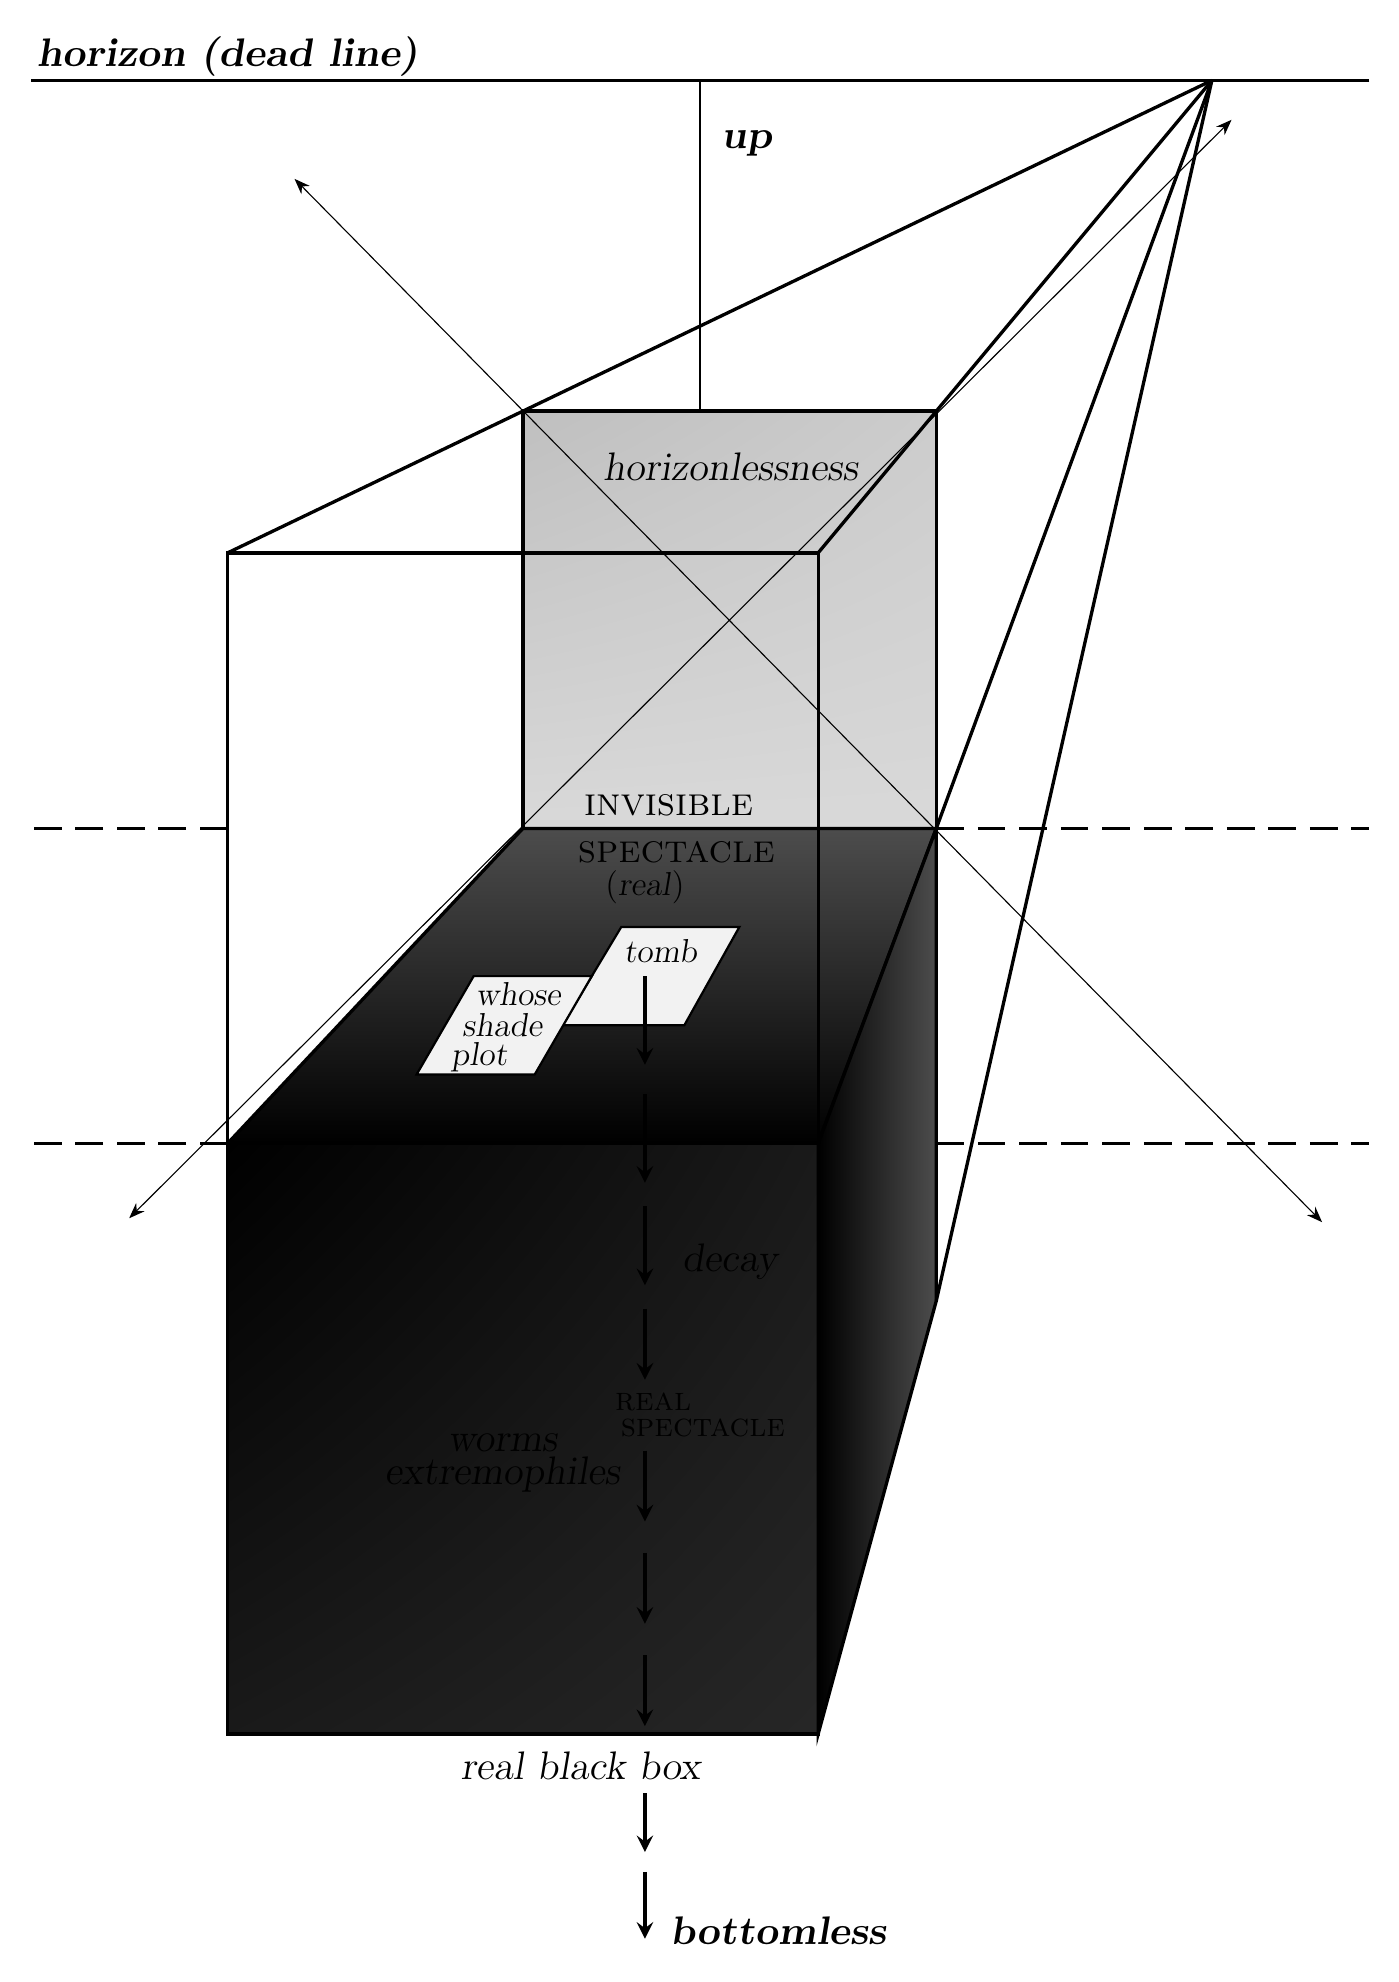
\begin{tikzpicture}
	%SQUARES
	\shade[upper left=gray!50,upper right=gray!40,lower left=gray!30,lower right=gray!30] 
	(-3.75,4) rectangle (1.5,9.3);	%top square (gray)
	\shade[bottom color=black,top color=black!70] (-7.5,0)--(-3.75,4)--(1.5,4)--(0,0)--cycle;
	%
	\draw[very thick] (-7.5,0)--(-3.75,4)--(1.5,4)--(0,0)--(-7.5,0);	%top parallelogram
	\draw[very thick] (-3.75,4) rectangle (1.5,9.3); %top, back
	\draw[very thick] (-7.5,7.5) rectangle (0,0);	%top, front
	%
	\shade[upper left=black,upper right=black!90,lower left=black!90,lower right=black!85] 
	(-7.5,-7.5) rectangle (0,0);
	\draw[very thick] (-7.5,-7.5) rectangle (0,0);		%lower square
	%
	\shade[left color=black, right color=black!70] (0,0)--(1.5,4)--(1.5,-2)--(0,-7.5)--(0,0)--cycle;
	\draw[very thick] (0,0)--(1.5,4)--(1.5,-2)--(0,-7.5)--(0,0)--cycle;	%side parallelogram
	%
	\filldraw[draw=black,fill=gray!10,thick] (-1.7,1.5)--(-1,2.75)--(-2.5,2.75)--(-3.25,1.5)--cycle; %right parallelogram
	\filldraw[draw=black,fill=gray!10,thick] (-2.875,2.125)--(-4.375,2.125)--(-5.1,0.875)--(-3.6,0.875)--cycle; %left parallelogram
	
	%DIAGONAL LINES
	\draw[very thick] (-7.5,7.5)--(5,13.5);
	\draw[very thick] (0,7.5)--(5,13.5);
	\draw[very thick] (1.5,-2)--(5,13.5);
	\draw[very thick] (1.5,4)--(5,13.5);
	
	%HORIZON LINES
	\draw[very thick] (7,13.5)--(-10,13.5);
	\draw[thick] (-1.5,9.3)--(-1.5,13.5);	%vertical
	\draw[very thick,dashed,dash pattern=on 10pt off 5pt] (1.5,4)--(7,4);
	\draw[very thick,dashed,dash pattern=on 10pt off 5pt] (-7.5,4)--(-10,4);
	%
	\draw[very thick,dashed,dash pattern=on 10pt off 5pt] (1.5,0)--(7,0);
	\draw[very thick,dashed,dash pattern=on 10pt off 5pt] (-7.5,0)--(-10,0);
	%
	\draw[{Stealth[length=2mm,width=1.5mm]}-{Stealth[length=2mm,width=1.5mm]}] (6.4,-1)--(-6.65,12.25);
	\draw[{Stealth[length=2mm,width=1.5mm]}-{Stealth[length=2mm,width=1.5mm]}] (-8.75,-0.95)--(5.25,13);
	
	%DOWNWARD ARROWS
	\draw[ultra thick,->,>=stealth] (-2.2,2.125)--(-2.2,1);
	\draw[ultra thick,->,>=stealth] (-2.2,0.625)--(-2.2,-0.5);
	%
	\draw[ultra thick,->,>=stealth] (-2.2,-0.8)--(-2.2,-1.8);
	\draw[ultra thick,->,>=stealth] (-2.2,-2.1)--(-2.2,-3);
	\node[align=left] at (-1.5,-3.45)  {\textsc{\large real}\\[-1mm]\textsc{\large $\,$spectacle}};
	\draw[ultra thick,->,>=stealth] (-2.2,-3.9)--(-2.2,-4.8);
	\draw[ultra thick,->,>=stealth] (-2.2,-5.2)--(-2.2,-6.1);
	\draw[ultra thick,->,>=stealth] (-2.2,-6.5)--(-2.2,-7.4);
	%
	\draw[ultra thick,->,>=stealth] (-2.2,-8.25)--(-2.2,-9);
	\draw[ultra thick,->,>=stealth] (-2.2,-9.25)--(-2.2,-10.1);
	
	%LABELS
	\node at (-7.5,13.8) {\Large \textbf{\textsl{horizon (dead line)}}};
	\node at (-0.9,12.7) {\Large \textbf{\textsl{up}}};
	\node at (-1.1,8.6)  {\Large \textsl{horizonlessness}};
	\node at (-1.9,4.3)  {\Large \textsl{\textsc{invisible}}};
	\node at (-1.8,3.7)  {\Large \textsl{\textsc{spectacle}}};
	\node at (-2.2,3.25) {\large (\textsl{real})};
	\node at (-2,2.45)	 {\large \textsl{tomb}};
	\node at (-3.8,1.9)  {\large \textsl{whose}};	%can't decipher original word
	\node at (-4.0,1.5)  {\large \textsl{shade}};
	\node at (-4.3,1.1)  {\large \textsl{plot}};
	\node at (-1.1,-1.5) {\Large \textsl{decay}};
	\node at (-4,-3.8)	 {\Large \textsl{worms}};
	\node at (-4,-4.2)	 {\Large \textsl{extremophiles}};
	
	\node at (-3,-7.9) {\Large \textsl{real black box}};
	\node at (-0.5,-10) {\Large \textbf{\textsl{bottomless}}};
	
	%\draw[help lines] (-5,-5) grid (5,5);
	\end{tikzpicture}
	
\end{document}